\documentclass[UTF8]{ctexart}
\usepackage{graphicx}
\usepackage{amsmath}
\pagestyle{plain}   
% \usepackage{booktabs}
% \usepackage{subfigure}
\usepackage{setspace}
\date{}
\title{DataStructureHW2实验报告} 
\author{杨景凯}
\date{2021/12/20} 
\begin{document} 
% \maketitle 
\begin{center}
    \quad \\
    \quad \\
    \quad \\
    \vskip 3.5cm
    \heiti \zihao{1} 跳表搜索长度探究\\
\end{center}
\vskip 3.5cm
\begin{quotation}
    \songti \fontsize{30}{30}
    \doublespacing
    \par\setlength\parindent{12em}
    \quad 
\begin{center}
    %学\hspace{0.61cm} 院:\underline{电子信息与电气工程学院}

    学生姓名:\underline{\qquad    \quad \quad 杨景凯    \quad  \quad\qquad }

    学\hspace{0.61cm} 号:\underline{\quad \quad\quad520021910550\quad\quad}

\end{center}
    
    \centering
    2022年3月1日
\end{quotation}
\clearpage
\tableofcontents
\clearpage
\section{相同概率下跳表长度对搜索长度的影响}
\subsection{理论分析}
跳表搜索长度是与跳表长度成正相关的。跳表能够向上建层,因此跳表搜索长度L与跳表长度l关系应该满足:
$$L\sim lg(l)$$
\subsection{实验证明}
我们抽取了跳表长度为10、20、50、100、200、500、1000的情况,每种情况下随机搜索10000次,做出下列折线图:
\begin{center}
    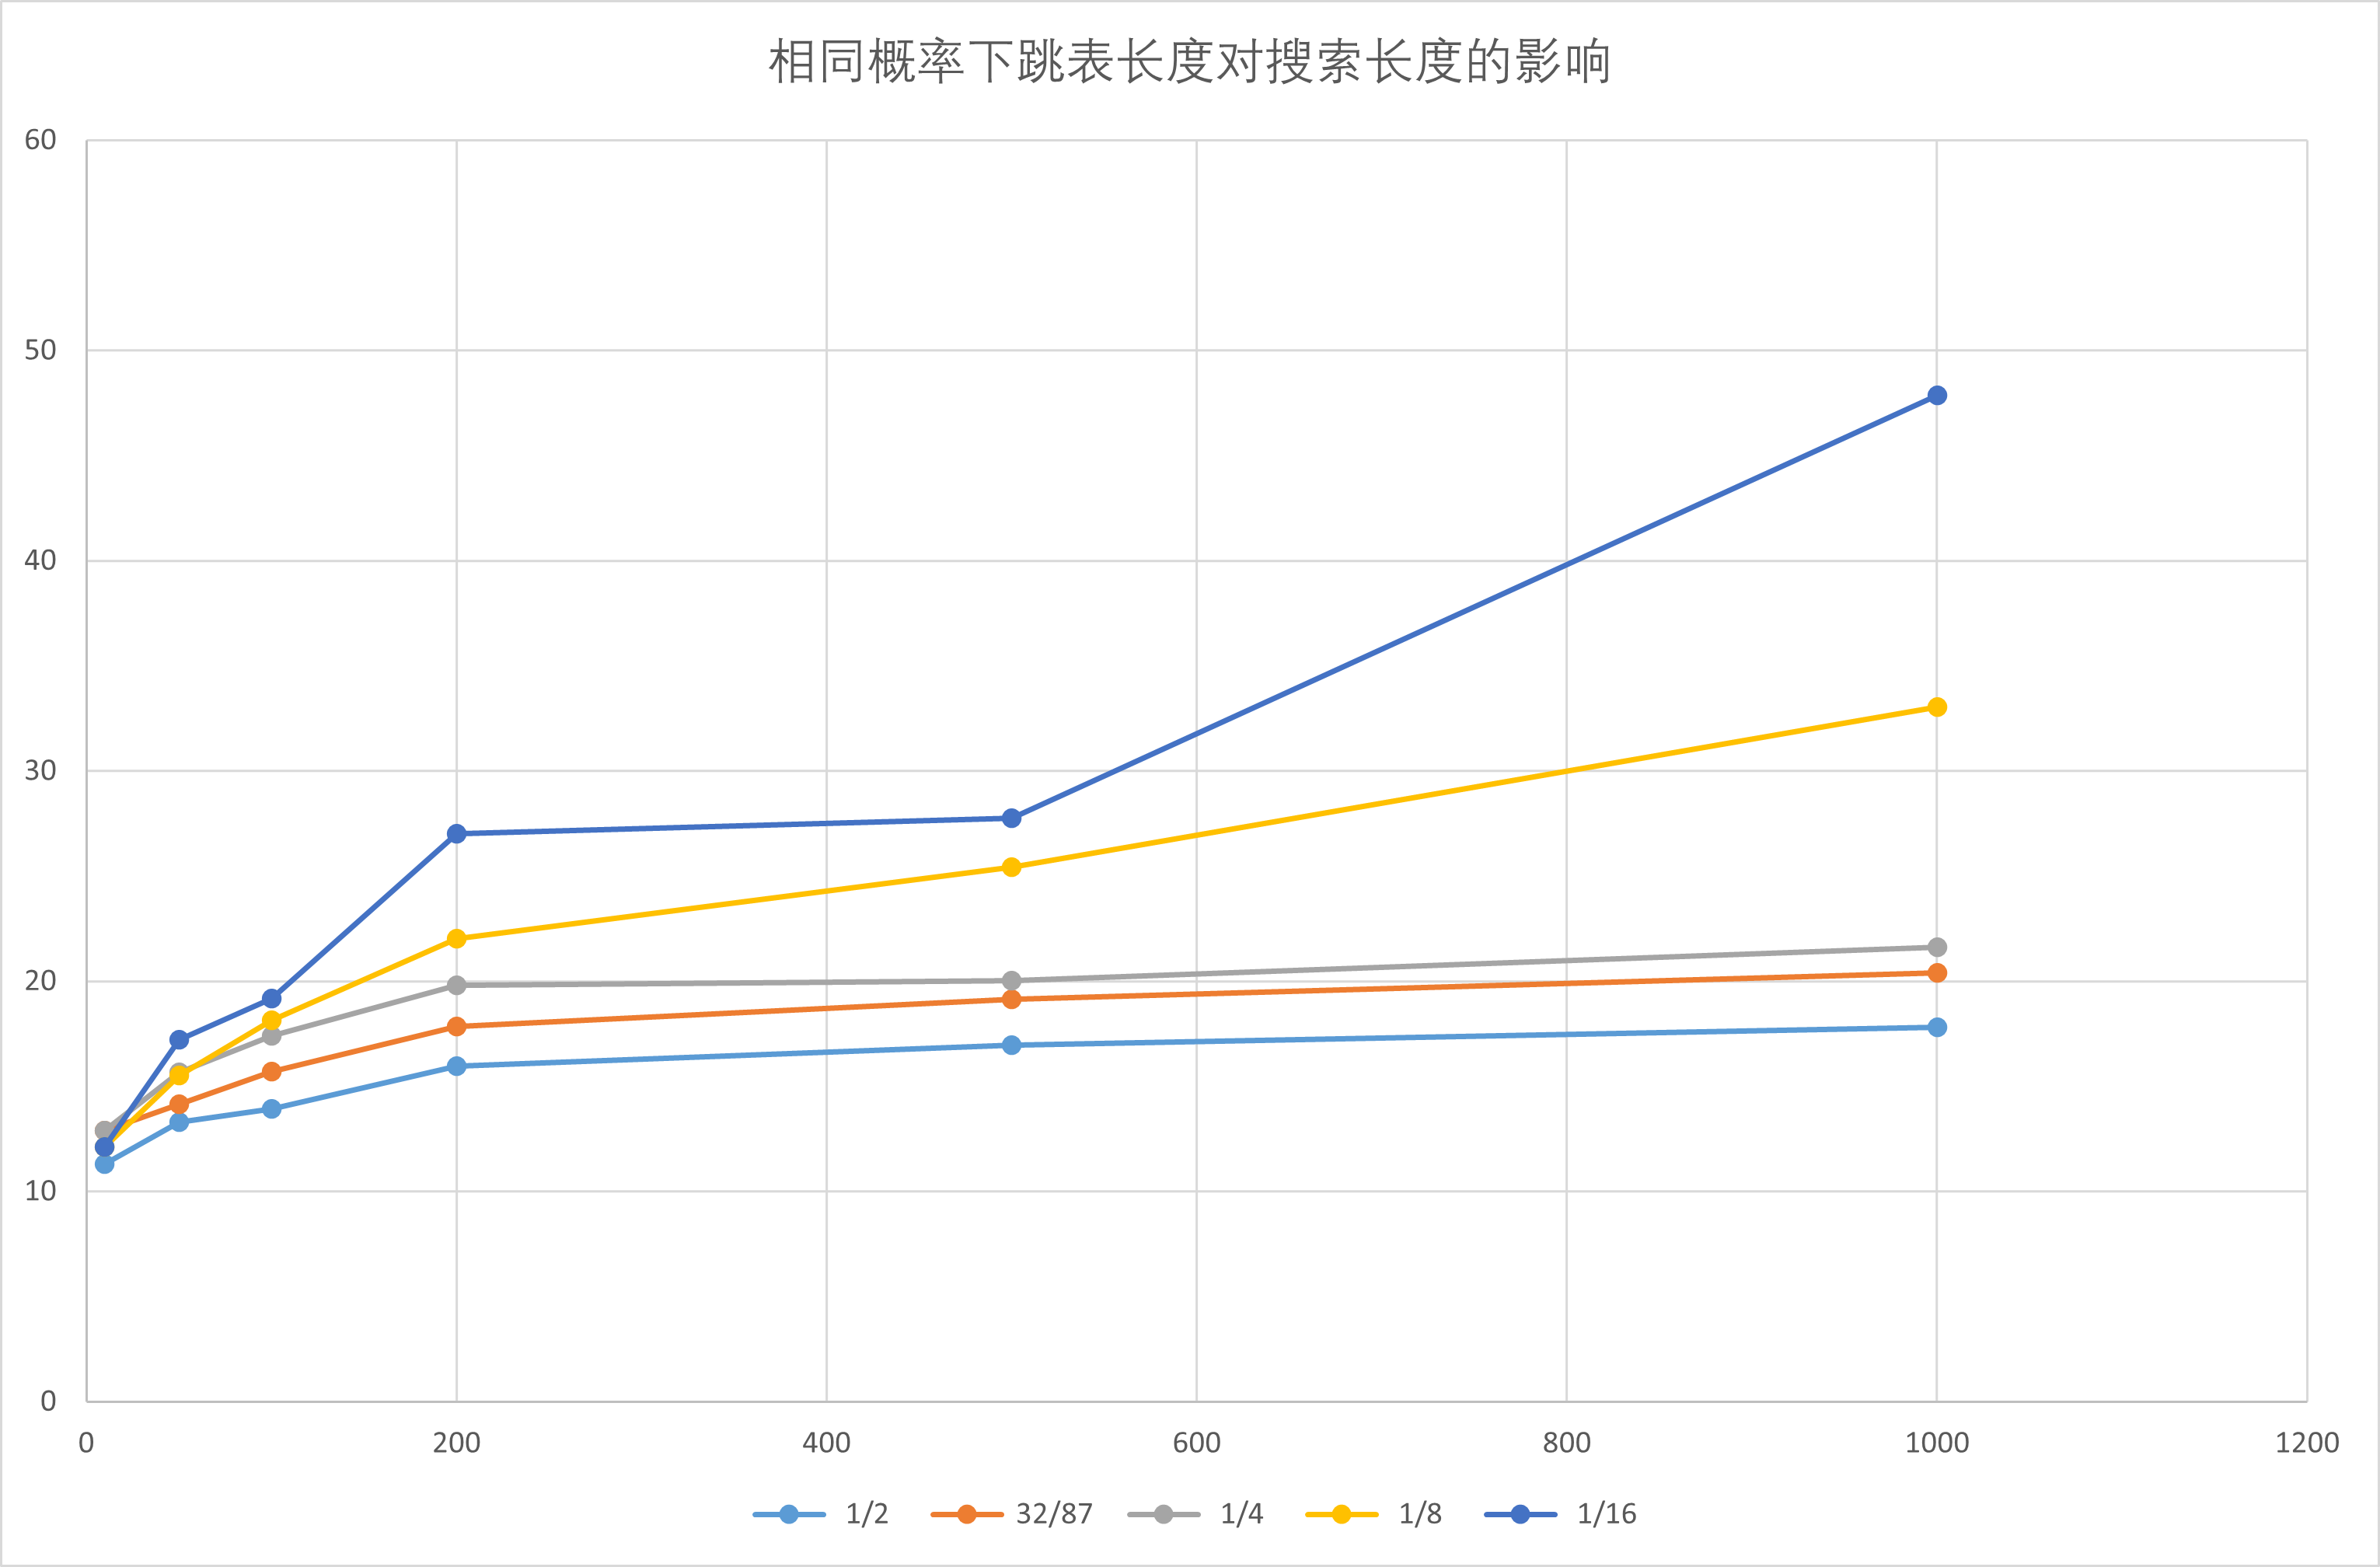
\includegraphics[scale=0.6]{Length.png}
\end{center}

由上图,随着跳表长度增加,跳表搜索长度增加,且随着跳表长度增加,跳表搜索长度增加速度降低。近似满足$L\sim lg(l)$关系。理论成立。

\section{相同跳表长度下概率对搜索长度的影响}
\subsection{理论分析}
跳表可以看成是一个对称的矩阵结构,因此,随着从0到1变化的概率,跳表搜索长度应该先减少后增加。因此,我们只探究了在0到$\frac{1}{2}$变化的情况。
\subsection{实验证明}
我们抽取了概率为$\frac{1}{2}$、$\frac{1}{e}$、$\frac{1}{4}$、$\frac{1}{8}$、$\frac{1}{16}$的情况,每种情况下随机搜索10000次,做出下列折线图:
\begin{center}
    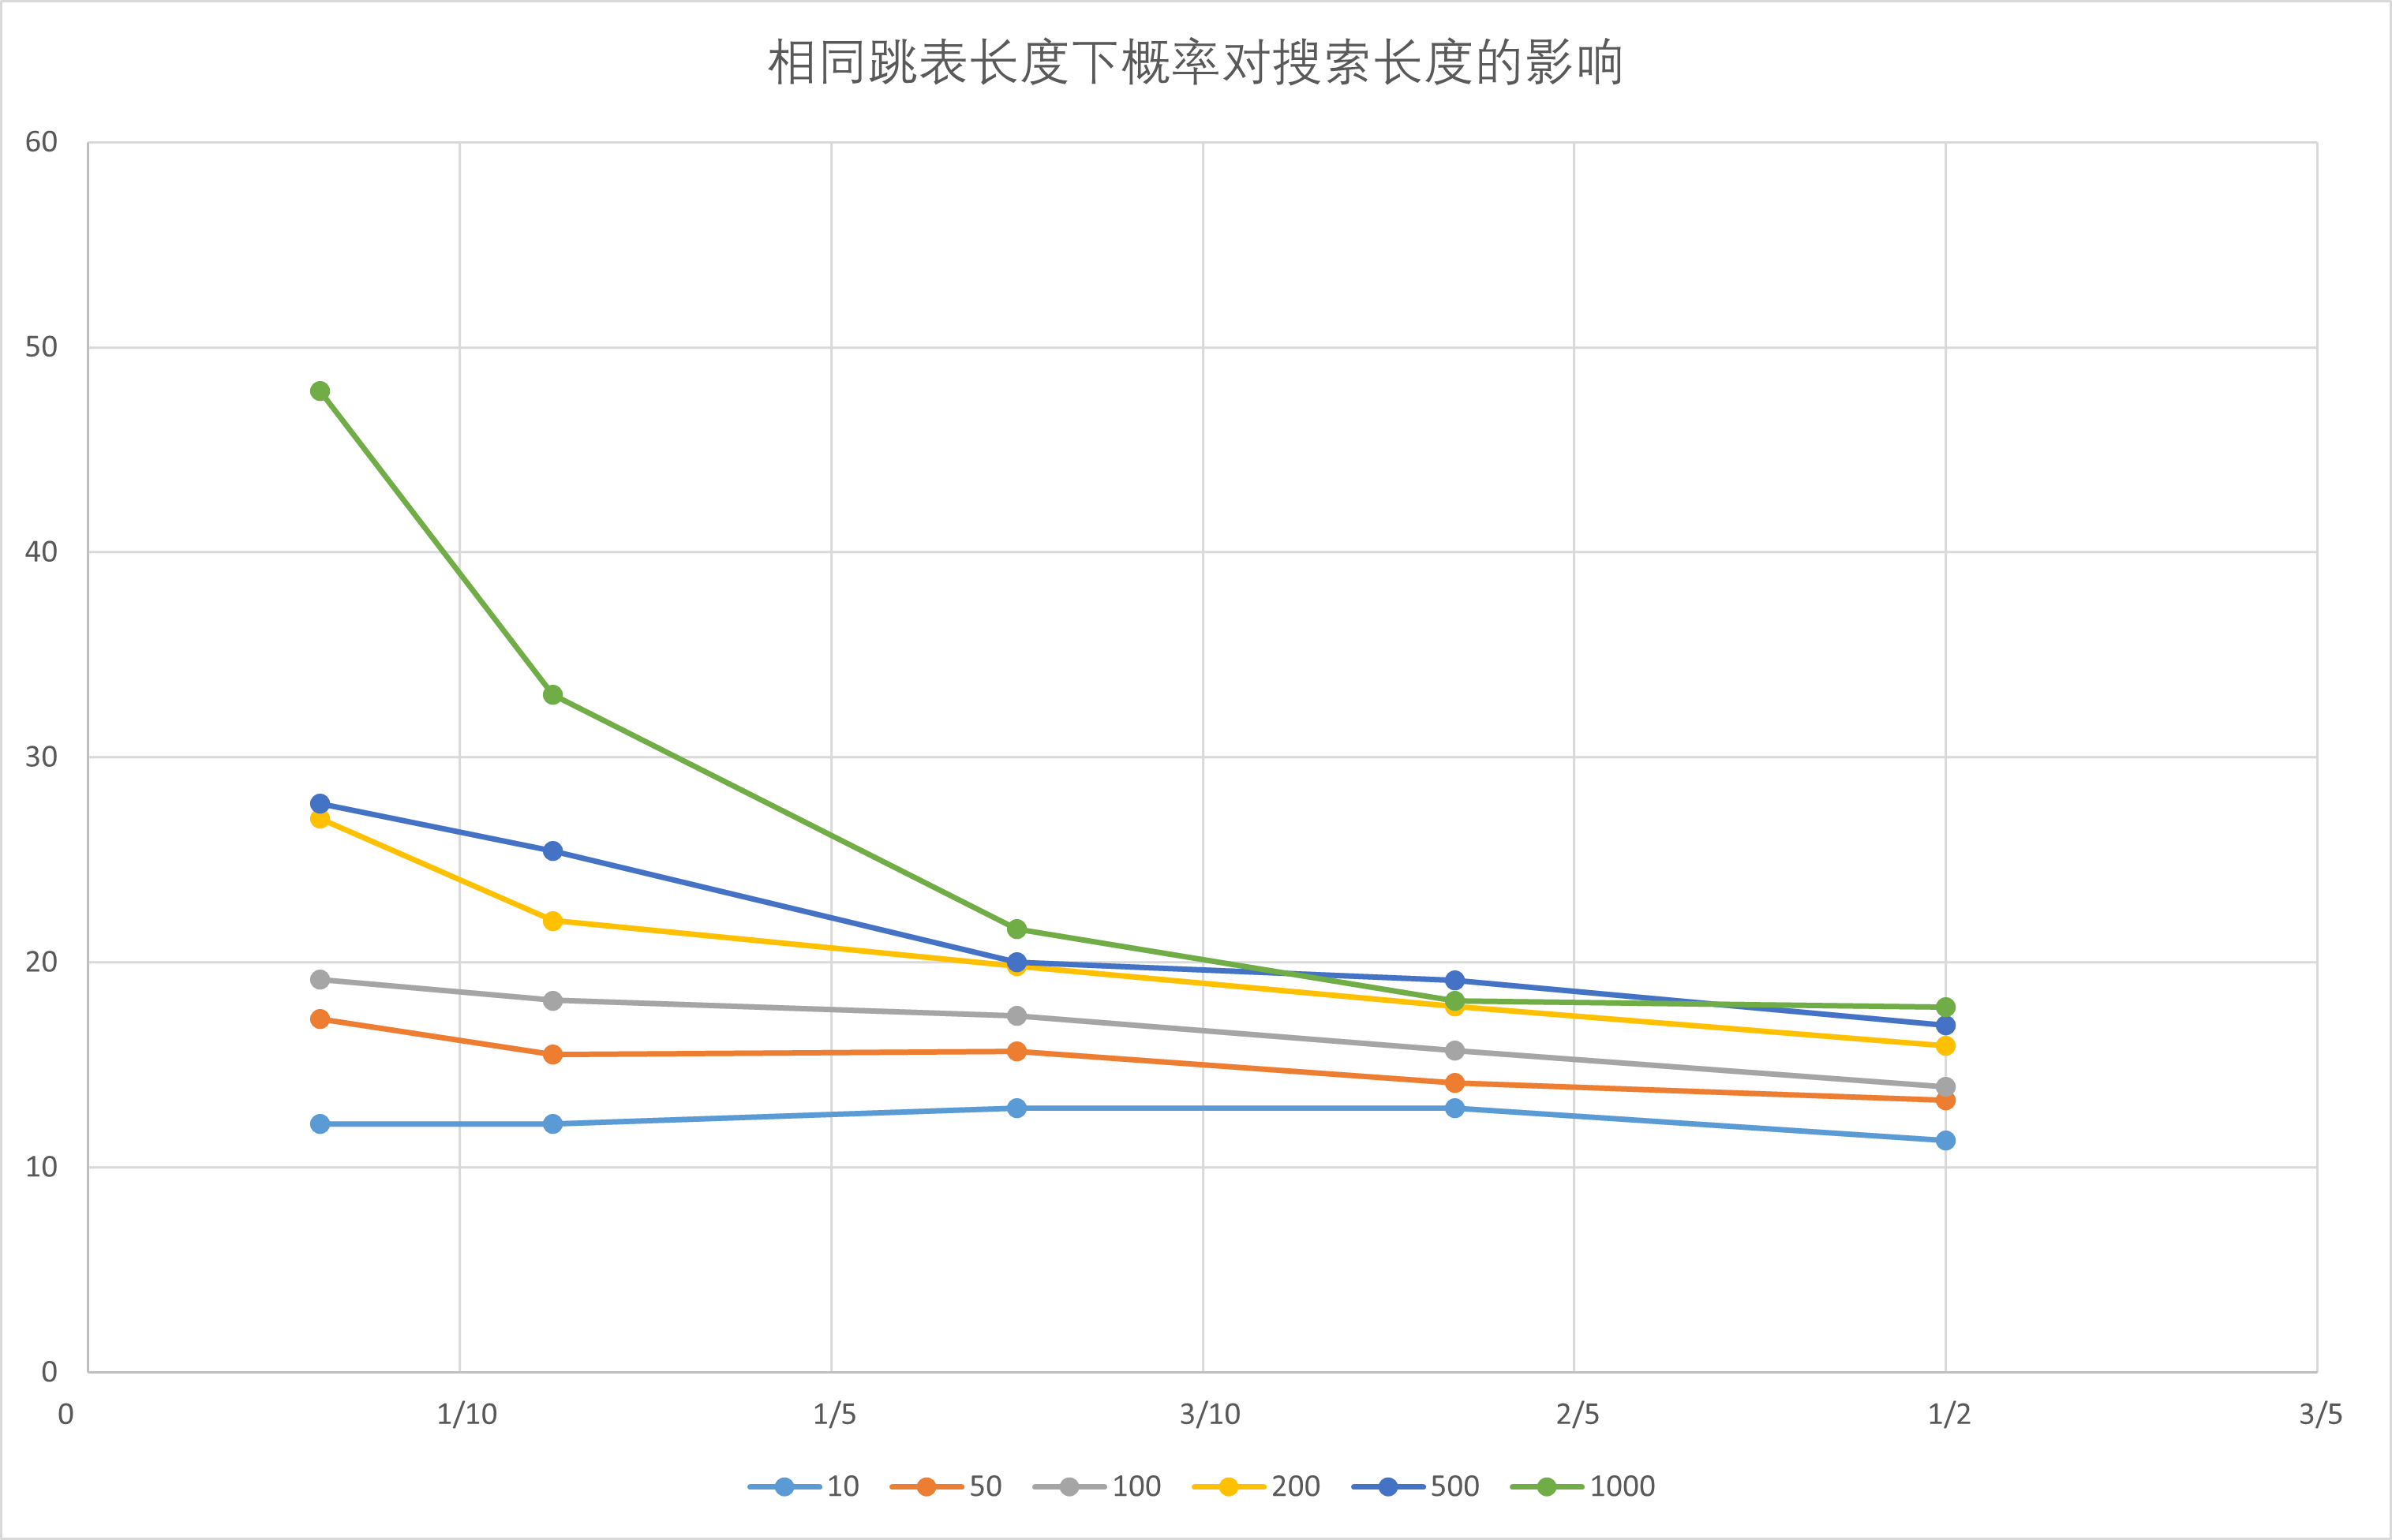
\includegraphics[scale=0.6]{Probility.png}
\end{center}

由上图,随着概率增加,跳表搜索长度减少。理论成立。

至于图中出现的一些偏差情况,我发现这些偏差主要出现于跳表长度较低的情况,我考虑了两种原因:
\begin{itemize}
    \item 搜索次数较少导致的误差\\
    对此假设,我增加了搜索次数,分别对20000次、50000次和100000次做了实验,发现与之前所得结果相差不多。因此,实验表明搜索次数较少不是导致此问题的根本原因。
    \item 跳表长度较短导致的误差\\
    由于不是第一点问题导致,考虑到在跳表长度较长时没有此问题,因此我认为这是导致误差的根本原因。
    当跳表长度较小时,由于概率问题,很容易使得在概率更高的情况下升高的跳表层数比概率更低时更低,或者是升高高度过高导致平均层数高于最高层数的一半,这些情况在跳表长度越低时越容易发生。这是导致在跳表长度较低时产生误差的根本原因。
\end{itemize}


% \clearpage
% \begin{thebibliography}{99} 
% \end{thebibliography}
\end{document}
